\chapter{Stato dell'arte}
\label{capitolo2}
\thispagestyle{empty}

\noindent
\section{Emergency management}

\vspace{0.5cm}

\begin{quotation}
{\footnotesize
\noindent{\emph{``The organization and management of resources and responsibilities for addressing all aspects of emergencies, in particular preparedness, response and initial recovery steps. Emergency management involves plans and institutional arrangements to engage and guide the efforts of government, non-government, voluntary and private agencies in comprehensive and coordinated ways to respond to the entire spectrum of emergency needs.''
} }
\begin{flushright}
United Nations International Strategy for Disaster Reduction (UNISDR)
\end{flushright}
}
\end{quotation}

\vspace{0.5cm}

\begin{quotation}
{\footnotesize
\noindent{\emph{``The managerial function charged with creating the framework within which communities reduce vulnerability to threats/hazards and cope with disasters.''
} }
\begin{flushright}
International Association of Emergency Managers (IAEM)
\end{flushright}
}
\end{quotation}

\vspace{0.5cm}

\noindent When a natural disaster occurs the emergency management is a crucial aspect to consider. Nowadays, thanks to technology progress, we can aim to improve this important process.
\\
\noindent Some natural disasters or accidents are unavoidable (e.g. floods, earthquakes), thus the only thing we can do is trying to mitigate their effects, be prepared, organize rescue and aid efforts as soon as possible. 
\\
\noindent The key to achieve these goals is information exchange and understanding, then the capability to process relevant information and coordinate actions in the shortest possible time.
\\
\noindent The ideal emergency plan should aim to prevent emergency from occurring, but this is not always possible as we said, so the plan must mitigate the results and effects of emergencies. As time goes on, more data can be collected and the plan should evolve. The development of an emergency plan turns out to be a cyclical process, where the important phases are the recognition and ranking of risks, the reaction, the reporting phase and the review of the risk management framework. At each iteration the plan is refined so as to have a better response for future events.
\\
\noindent During an emergency, communication can be difficult for various reasons. In order to develop an effective management plan we need to collect enough relevant information in some way. Latest technologies can help us a lot to obtain real time and semi-real time information, for example satellite technologies like imagery and GPS, IOT devices and Internet. The latter is really important, because it is the main channel through which common people can interact with, in particular thanks to Social Media.
\\
\noindent These sources of information can be all helpful, but they need to be integrated each other to achieve better performance and provide real time information that can be crucial during extreme events.
\\
\noindent We can say that the keys for success are information and coordination.

\subsection{Emergency cycle}
An emergency management process is typically represented as composed by four cyclical phases: preparedness, response, recovery and mitigation. The distinction among these four phases permits to plan in the best way possible the strategies apt to minimize damages and to restore, as quickly as possible, the normal situation.

\begin{figure}[h]
    \begin{center}
      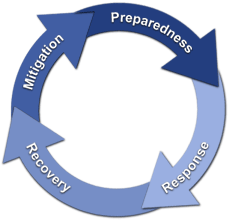
\includegraphics[width=5cm]{img/emergencyCycle.png}
      \caption{Four Phases of Emergency Management (NEHRP, 2009)}
      \label{fig:emergencyCycle}
    \end{center}
\end{figure}
\vspace*{0.3cm}

\subsubsection{Preparedness}
Objective of this phase is to develop an ability to respond in a proper way when a disaster occurs, in order to be capable to minimize damages. For this reason, this phase take place before an emergency occurs. In this step governments, organizations and individuals develop plans so as to anticipate problems that are likely to emerge in future disaster situation and facilitate response to emergencies. Obviously there is in some case the necessity to testing and exercising those plans.
\\
Evacuation plans, installation of sensors, posting emergency telephone numbers and training personnel are examples of preparedness activities. 

\subsubsection{Response}
Is the phase that begins when an emergency occurs or, if the event is predicted, immediately before the event. During this phase, preparedness plans studied in the previous phase are executed, emergency services are mobilized (e.g., firefighters, ambulance, police, or others), evacuations are performed and emergency shelters are constructed. The goal of this phase is to save lives, limitate property damages and establish the level of damage. During or at the end of the response phase is possible to evaluate the plan adopted and think about possible corrections that can improve it for any subsequent event. 

\subsubsection{Recovery}
Recovery phase take place immediately after the emergency. The goal of this phase is to bring the affected area to a normal or improved situation. Recovery activities can be divided into short-term recovery activities and long-term recovery activities. Short-term recovery activities comprehend those activities that are intended to restore community's system to the minimum operating standard (e.g., cleanup, temporary housing). Long-term recovery activities comprehend the rebuilding and improving of the affected area (e.g., rebuilding of roads, rebuilding of bridges, rebuilding of houses) and restoring economic activities. The aim of long-term activities is to stabilizing the system and preventing the reoccurrence or, in case of unavoidable event, prepare it to face a future emergency in the best possible way.

\newpage
\subsubsection{Mitigation}
\begin{quotation}
{\footnotesize
\noindent{\emph{``Policies and actions taken before an event which are intended to minimize the extent of damage when an event does occur.''
} }
\begin{flushright}
Drabek, Mushkatel, and Kilijanek, 1983:12
\end{flushright}
}
\end{quotation}
Mitigation is the end phase of the process. It is a long-term phase during which risk analysis is performed and mitigation measures are taken to eliminate or reduce the damaging effects to human life and property from hazard and their effects. 
\\
\noindent Make structure disaster-resistant, constructing barriers such as levees, changing building standards and modification of existing structure to make them more resistant to seismic activities are all mitigation actions.
\vspace*{0.3cm}
\\
After the mitigation phase, a new cycle begins. 
\\
Even if the four phases may appear separated from each other, they actually overlap and merge.

\newpage
\subsection{Hazard}
An hazard is defined as a:

\begin{quotation}
{\footnotesize
\noindent{\emph{``Source of danger that may or may not lead to an emergency or disaster and is named after the emergency/disaster that could be so precipitated.''
} }
\begin{flushright}
National Governors Association, 1982
\end{flushright}
}
\end{quotation}

\noindent During an emergency event, the efforts of one or more of the emergency services (e.g., firefighters, ambulance, police, or others) are required in order to manage it. In case that the event is so critical and the emergency services are not sufficient to deal with it, the event is classified as a disaster.

\subsubsection{Natural Hazards}

\begin{quotation}
{\footnotesize
\noindent{\emph{``Natural hazards are natural events that threaten lives, property, and other assets. Often, natural hazards can be predicted. They tend to occur repeatedly in the same geographical locations because they are related to weather patterns or physical characteristics of an area. ''
} }
\begin{flushright}
Federal Emergency Management Agency (FEMA)
\end{flushright}
}
\end{quotation}

\noindent Natural hazards such as earthquakes, landslides, floods, tsunamis and volcanic eruptions affect every year human and animal lives and properties all around the globe and, in many cases, the reasons are not in our control. In some cases human activities and development have increased natural hazards (e.g., construct buildings on an earthquake zone without taking appropriate precautions, building communities in floodplain, or others).

The following are large scale hazards and are those that particularly influence people's life :

\begin{itemize}
	\item \textit{Flood:} high-water stage in which water overflows its natural or artificial banks onto normally dry land, such as a river inundating its floodplain. Floods can be slow or fast-rising, but generally develop over a period of days. Flood may be caused by a number of factors, including heavy rainfall.
	\item \textit{Earthquake:} any sudden shaking of the ground caused by the passage of seismic waves through Earth's rocks. Seismic waves are produced when some form of energy stored in Earth's crust is suddenly released, usually when masses of rock straining against one another suddenly fracture and ``slip''. Earthquakes occur most often along geologic faults, narrow zones where rock masses move in relation to one another. Earthquakes can cause buildings and bridges to collapse; disrupt gas, electric and phone service; and sometimes trigger landslides, avalanches, flash floods, fires, and tsunamis. Over the centuries they have been responsible for millions of deaths and an incalculable amount of damages to properties.
	\item \textit{Tropical cyclone:} also called typhoon or hurricane, an intense circular storm that originates over warm tropical oceans and is characterized by low atmospheric pressure, high winds, and heavy rain. Drawing energy from the sea surface and maintaining its strength as long as it remains over warm water, a tropical cyclone generates winds that exceed 119 km (74 miles) per hour. In extreme cases winds may exceed 240 km (150 miles) per hour, and gusts may surpass 320 km (200 miles) per hour. Accompanying these strong winds are torrential rains and a devastating phenomenon known as the storm surge, an elevation of the sea surface that can reach 6 metres (20 feet) above normal levels. Such a combination of high winds and water makes cyclones a serious hazard for coastal areas in tropical and subtropical areas of the world. Every year during the late summer months (July-September in the Northern Hemisphere and January-March in the Southern Hemisphere), cyclones strike regions as far apart as the Gulf Coast of North America, northwestern Australia, and eastern India and Bangladesh.
	\item \textit{Tornado:} a small-diameter column of violently rotating air developed within a convective cloud and in contact with the ground. Tornadoes occur most often in association with thunderstorms during the spring and summer in the mid-latitudes of both the Northern and Southern Hemispheres. These whirling atmospheric vortices can generate the strongest winds known on Earth: wind speeds in the range of 500 km (300 miles) per hour have been measured in extreme events. When winds of this magnitude strike a populated area, they can cause enormous destruction and great loss of life, mainly through injuries from flying debris and collapsing structures.
	\item \textit{Tsunami:} also called seismic sea wave or tidal wave, catastrophic ocean wave, usually caused by a submarine earthquake, by an underwater or coastal landslide, or by the eruption of a volcano.	
	\item \textit{Landslide:} also called landslip , the movement downslope of a mass of rock, debris, earth, or soil (soil being a mixture of earth and debris). Landslides occur when gravitational and other types of shear stresses within a slope exceed the shear strength (resistance to shearing) of the materials that form the slope. Shear stresses can be built up within a slope by a number of processes. These include oversteepening of the base of the slope, such as by natural erosion or excavation, and loading of the slope, such as by an inflow of water, a rise in the groundwater table, or the accumulation of debris on the slope's surface. Short-term stresses, such as those imposed by earthquakes and rainstorms, can likewise contribute to the activation of landslides.
	\item \textit{Volcanic eruption:} eruptions of molten rock, hot rock fragments, and hot gases from the surface of the earth that are ejected to heights and spread for several miles.
\end{itemize}

\newpage
\section{Geographic Information System}
Geographic information systems (GIS) are combined hardware and software systems for the capture, storage, checking, integration, manipulation, display and analysis of spatially referenced (geocoded) data. The data (i.e., information with coordinate referencing, such as latitude and longitude) are input into these systems and displayed in two or three dimensional maps and other diagrammatic forms.
GIS is a computer system for performing geographical analysis by fusing spatial data from different sources and analyze spatial patterns that may be present.

\section{The Copernicus System}
\noindent Nowadays there is not a standard system to manage emergency, however many different project exist. We take into account the Copernicus Emergency Management Service, which is an EU programme aimed at developing European information services based on satellite Earth Observation and in situ (non space) data~\cite{copernicus}.
\\
\noindent Copernicus has a series of services ranging from monitoring land, sea and atmosphere, support climate change mitigation and in particular management of emergency situations. Copernicus EMS consists of the Mapping Service (in activity since 1st April 2012) and the Early Warning System for floods.
\\
\noindent The information provided by Copernicus are freely and openly accessible to its users, which are mostly public authorities.
\\
\noindent Copernicus EMS since 2012 is running the following operations.

\begin{itemize}
\item   Copernicus EMS Rapid Mapping (RM)

        provides information about the extent and impact of disasters (natural or manmade) to European Civil Protection Authorities and to International Humanitarian Aid organizations. The information has an high quality, is reliable and timely.
        
\item   Copernicus EMS Early Warning European Forest Fire Information System (EFFIS)

        provides data on forest fires in Europe, Middle East and North Africa, these data can be near real-time and also historical data. Information range from pre-fire conditions to assessing post-fire damages.
        
\newpage

\item   Copernicus EMS Risk \& Recovery (R\&R)

        provides geo information to support decision for prevention, preparedness, disaster risk reduction and recovery phase of a crisis (e.g. reconstruction planning).
        
\item   Copernicus EMS Early Warning European Flood Awareness System (EFAS)

        support national hydrological services providing added value information, it produces also a unique overview on the current and forecast flood situation and send the data to competent authorities like Emergency Response and Coordination Centre (ERCC).
        
\end{itemize}

\noindent The system presented however is not perfect, in fact it is currently facing specific challenges and operational gaps.
\\
Starting from the Mapping Component we can say that the main source of data used by EMS are satellite images acquired on purpose following a map request. Timeliness is one of the main user requirements of the EMS and this is not yet fully achieved. In fact it is not unusual to experience delays up to 72 hours while users have expressed the requirement of receiving first crisis information within the first 24 hours after the disaster. Many factors are the cause of this delay, for example satellite orbital constraints and bad weather conditions preventing the collection of optical images. Moreover in case of large scale disasters map production throughput could be insufficient to timely analyze the affected area. Lastly satellite based emergency maps have also limitations in quality.
\\
Regarding the Early Warning Component at the current state it can access weather prediction up to 15 days in advance, but forecasts are still subject to relatively high uncertainties. Forecast verification is also an important aspect to improve, it is normally done through event based verification, assessing hit, false alarm and misses for each event. Currently events are assessed through feedback reports and media. Another important aspect is historical data availability, it is a key point to improve the Early Warning System and provide realistic impact estimation.

\newpage
\section{Social Networks and Emergency Management}
\noindent This section discuss Social Networks and the role they play in emergency management.
\\
\noindent First of all we will present a general introduction to SN, explaining what they are and why they are so important nowadays. We will focus in particular on Twitter and explain why it suites our application case.
\\
Later we will introduce the concept of crowdsourcing, which is strongly related to Social Networks, deepening its use in the context of emergency management.

\subsection{Social Networks}
\noindent Social Networks are Internet services that allows the management of social relations and communications. They host a lot of users and their social bonds, for example friendship or family relationships. Typically these services are available through browsers or mobile applications. These services were born in the late 90's and became popular in the early 2000s, they allow the user to create a profile page, a contact list and publish a stream of updates visible to others. One of the main characteristic of Social Networks is that they allow users to generate content (text, multimedia, etc...) and this is very important because it was the starting point of the digital revolution of Web 2.0.
\\
The study of Social Networks is conducted by various disciplines. This research over different approaches has pointed out the way how Social Networks work, over multiple levels, ranging from families to national communities. It has been shown that SN play a crucial role in problem solving and management systems of organizations, moreover they can help individuals to achieve their objectives.
\\
Mathematically speaking, SN can be described by models that use graph theory. In these representations, subjects which can be individuals, groups or communities are the nodes and they can be connected by arcs that represent the relationships among them. Relationships can be univocal (like a following relation) or biunique (like a friendship relation), Social Networks that implements the first kind of relation tend to be more 'open', for example on Twitter, by default, everyone can follow everyone (even famous people) without an explicit consent.
\\
The social network has its own density, which is a parameter which ranges from 0 to 1 and expresses the general level of cohesion of the links between the points of a given graph. The density of a graph that represents a social network can be an indicator of the efficiency in the exchange of information and usefulness for individuals. However, small and dense networks can be less useful than weak tied networks, because the latter can be more flexible leading itself to a better exchange of ideas and opportunities. The Dunbar's number states that the size of a social network able to support stable relationships are limited to about 150 members. These are relationships in which an individual knows who each person is and how each person relates to every other person. This number has been obtained through sociology and anthropology studies, it can be viewed as a kind of limit for the human beings to recognize members of a group and keep track of events. We can also argue that too large groups can be bad, because they have a larger probability to contain noisy elements.

\subsection{Twitter}
\noindent Twitter is one of the most widespread social network sites worldwide. It is an online free social networking and microblogging service, it allows users to publish text messages of up to 140 characters, which are called ``tweets''. Twitter is entirely based on an Open Source architecture~\cite{twitteropensource}.
\\
\noindent Every user have a personal profile which he can update through status messages, these updates can be done through Twitter website, via SMS or various applications based on Twitter's API~\cite{twitterapi}. Status updates become immediately available for all the users that ``follow'' the user who posted the tweet. In fact the relationship between users is unidirectional of ``follower/following'' with this characteristics:

\begin{itemize}
    \item a user can see all the status updates and personal profile pages of all the ``following'', which are the users that he follows. He can comment (mention, @) or share (retweet, RT) a specific tweet they have posted before.
    \item the user's personal profile and all its status updates are visible only by his ``followers'', which are users that have decided to follow him.
\end{itemize}

\noindent Twitter has become really popular, despite Facebook, thanks to its simplicity and ease of use. In Twitter there is not the concept of conversation as in other social networks, however it is possible to send private messages to other users and it is possible to group tweets through the use of ``hashtags'' (\#). Hashtags define the topic of the discussion and help in the search of all recent tweets which refer to it.
The search can be performed by keyword and will return a series of public posts from different users, regardless of the fact that who has done the search is their follower or not. Thanks to this feature we can say that Twitter is a kind of journalistic social network, which has become the main platform to spread news all around the world.

\subsection{Crowdsourcing}

\begin{quotation}
{\footnotesize
\noindent{\emph{``Crowdsourcing is a type of participative online activity in which an individual, an institution, a non-profit organization, or company proposes to a group of individuals of varying knowledge, heterogeneity, and number, via a flexible open call, the voluntary undertaking of a task. The undertaking of the task, of variable complexity and modularity, and in which the crowd should participate bringing their work, money, knowledge and/or experience, always entails mutual benefit. The user will receive the satisfaction of a given type of need, be it economic, social recognition, self-esteem, or the development of individual skills, while the crowdsourcer will obtain and utilize to their advantage that what the user has brought to the venture, whose form will depend on the type of activity undertaken.''
} }
\begin{flushright}
Est\'elles et Gonz\'alez, 2012~\cite{estellesgonzalez}.
\end{flushright}
}
\end{quotation}

\noindent Crowdsourcing can be seen as a model of production and troubleshooting, where the solution is built by an undefined group of people, the ``crowd'', who meet online. People who have helped to find the solution can be payed with money or prizes or intellectual satisfaction. Crowdsourcing is so powerful thanks to the ``Wisodm of the crowd'', that is the idea that a collective opinion of a group of individuals is more accurate than the one of a single expert.
\\
Crowdsourcing has many advantages with respect to traditional problem solving models. First of all, low cost solutions can be found, in fact the payment is based on result and sometimes it not even expected. Organizations which use this model can receive suggestions from a much more wider pool of contacts with respect to their primary network of contacts, moreover they can understand their consumers needs.

\subsubsection{Crowdsourcing and emergency phases}

\noindent During the \textbf{Preparedness} phase, citizens can provide useful information, for example informing the authorities about the risk level of the territory and pointing out dangerous infrastructures. All these information can be helpful during the creation of an emergency plan. Moreover, during this phase is useful the activation of a series of tools that tell the citizens what to do in case of emergency, which is called ``crowdfeeding''.
\\
\noindent The \textbf{Response} phase is the most critical, thus information provided by citizens can help strategic decisions. Information can provide a general description of the territory, information about citizens affected by the event or help requests.
\\
\noindent Crowdsourcing is also useful to better understand what are the necessary intervention for the rebuilding process during the \textbf{Recovery} phase. Also authorities can use it to consult external experts to solve problems that can emerge in this phase.
\\
\noindent Lastly, in the \textbf{Mitigation} phase, the crowd can be used to gather complaints and social problems arising from the event.

\vspace{0.5cm}
\subsection{Social Network for Emergency Management - Examples}

\noindent In this section we will present some significant examples that show a concrete application of social networking technologies and crowdsourcing to the management of natural disasters and extreme events.

\subsubsection{Colorado floods}
\noindent Researchers of the PennState university investigated the use of social media applied to emergency management, in particular their ultimate goal is to quickly identify impacted areas in need of assistance following a natural disaster. They analyzed the September 2013 Colorado floods using a combination of remote sensing techniques to identify flooded areas, using Twitter and Flickr as sources of information.
\\
\noindent When a disaster occurs, response teams typically prioritize rescue and aid efforts to regions that are affected the most, to identify this areas public satellite imagery is used. The main problem here is that satellite imagery for a location is not always available in a timely manner and sometimes it take a long time to become available, even several days. The purpose of the study is to show that social media can be used to fill the gaps in the satellite data.
\\
\noindent The disaster occurred in an urban area, so the researchers were able to access hundreds of thousands tweets from people affected by the flooding.
Subsequently all the amount of data was analyzed, both text tweets and images. Tweets of interest mention a ``river in the road'' or similar sentences, so it is a search by keywords. For images the analysis process is more difficult and interesting, in fact researchers developed a machine-learning algorithm to automatically analyze several images to identify individual pixels of images that contained water.
\\
\noindent In this specific study case, looking only at satellite imagery downtown Boulder showed very little flooding, but analyzing the social media information they realized that many areas were underwater. An interesting example is a picture of a partially submerged truck, the picture took from the satellite has low quality and you can barely identify the object, the same truck is also the subject of a picture uploaded on Flickr by a citizen, this picture is much more detailed so that you can identify the vehicle and even see if there is someone stuck in.
\\
\noindent This research had positive feedbacks and now researchers are improving the algorithms used and assessing whether they can be applied to future flooding events~\cite{pennstate}.

\subsubsection{Italian Earthquakes}
\noindent Another interesting study case is about the application of Social Sensing in the context of Emergency Management. Social Sensing is based on the idea that groups of people can provide a set of information similar to those obtainable from a single sensor, this generates an amount of information that can be collected and analyzed subsequently.
\\
This particular study focuses on a novel and general architecture for an early warning system, which is a system able to timely detect events that are of social concern. To develop the system they used Twitter as source of information for the detection of earthquakes on the Italian territory. This study comes from the idea that the first people who announce such phenomena are those directly involved in the event. It leverages Social Networks, a particular type of Social Media suited to this type of analysis due to the large number of users involved and their high level of interaction. Moreover they used Twitter because it is the SN which is best suited to Social Sensing thanks to its features, for example the structure of the Tweet (max. 140 characters length), the lifetime of Tweets and the responsiveness of the platform.
\\
The project proposes a modular architecture, the first steps are data acquisition and filtering, which are used to build a filtered data set that contains only relevant information. Then there are the event detection and damage assessment modules, they are in charge of detect spatial and temporal location of the event and also determine the impact and the consequences of an emergency on community infrastructures.
\\
The architecture described has been tested with italian earthquakes data, but it turned out to be general enough to manage any kind of emergency. Finally they made an interesting observation about security issues which are not taken into account in this study, leaving this option open for future works~\cite{italianearthquakes}.

\subsubsection{Hurricane Sandy}
\noindent An interesting case of study is about the integration between Twitter data and nightlight satellite imagery for access area with power outages during a natural hazard. This case of study is based on the Hurricane Sandy that in 2012 hit the Eastern seaboard of the United States in the area of New Jersey and New York. In particular, in this study they assessed that by the fusion of social media with nightlight remote sensing imagery, they are able to detect power outages at a street-level resolution. 
\\
In this study, a GIS (Geographical Information System) was used to compare the spatial aggregation of the vector point of tweets to the raster-based satellite imagery.
\\
In order to use satellite imagery for this purpose, it is necessary to compare previously collected nightlight imagery of normal condition with new clear imagery collected immediately after the hurricane. Doing this is not so simple because of significant cloud coverage from the storm and the fact that nightlight imagery is available at a low temporal resolution due to the uniqueness of the satellite collection and its orbit. In addition, changes in nightlight levels can occur for other reasons, thus it is important to have temporally comparable imagery to limit, for example, seasonal variation.
\\
If there are clear and temporally comparable imagery from the satellite, analysis of change in light emission occurring due to the event is performed between the ``before'' and ``after'' satellite images in order to produce a brightness difference raster in which the red color identifies most significantly power outages.
\\
Using only remote imagery cannot assess human condition. For these reason, also data from Twitter were collected, basing the search on power outage keywords in order to supplement imagery when it is not available[12].
\\
After an analysis of the tweets, it can be noted that there are more tweets using power related key terms within the affected area with respect to outside the extent.
\\
An argument in favor of collecting data from social media in order to supplement remote sensing data could be the fact that the former are available at high temporal resolution but with sparse spatial resolution unless aggregated, while the latter are available with high spatial resolution, coverage dependent on atmospheric conditions and can only be collected within few hours.
\\
Obviously, the method descripted above is particularly effective where there is a large amount of data from social media. Social media for natural disasters is increasingly used as a source of information from a population, especially in urban areas~\cite{hurricanesandy}.

\subsubsection{Floods in Philippine and Pakistan}
\noindent The results of the disaster response depends on how fast information about location, timing and impact of the event are retrieved.

\noindent Typically, this information reaches humanitarian organizations only after many hours or several day and is not capable to capture the three key parameters discussed before.
For this reason, in order to achieve a better quality in the response phase, data from different near-real-time sources are mixed together (e.g., observation of water coverage from satellite, flood related social media activity from Twitter). 

\noindent Whereas information by satellite cannot be always retrieved and has often a delay of 24h or more, data streams from social network are available within few minutes of publication. 
Given the speed with which data from social media can be retrieved and the possibility to extract the geographic location of posts from gps data or from the body text (e.g., mention of ``New York''), it is possible to link these posts to the location on a map. 

\noindent One of the first time in which this system has been used is after the Haiti's earthquake in 2010. Since then, social media are been used regularly during or after disasters for a rapid mapping of it. 
One of the obtained results from this method, is that is possible to delineate earthquake-affected areas within several minutes, before official earthquake observations are available.

\noindent This paper discuss case-studies based on floods in Pakistan and Philippines with the aim to provide a comparison between different channels of early detection information in terms of the timing of the signals, the type and the value of information. These channels are: data from the near-real-time satellite flood detention system (GFDS) and social media reporting through Twitter.
The paper highlights that both the GFDS satellite data and the Twitter data have huge potential for enhancing disaster response, whereas both also have issues.

\noindent As regards GFDS satellite information, this is suited for monitoring and measuring large riverine floods and less so for small floods of short duration. In addition to this, there are some highlighted errors like: 
\begin{list}{-}{}
	\item in agricultural areas irrigation measurement and comparison pixels can affect the signal;
	\item snows gives a similar signal as water and is not filtered out in the version analyzed in the study.
\end{list}
For that reason, GFDS may give erroneous results in coastal areas and GFDS signal is less suited for use in delta regions and islands.

\noindent On the other hand, in contrast to the GFDS signal, Twitter can be used for monitoring floods of any size as long as the observations and discussions are shared by people on social media. 
Furthermore, the analysis of Tweets has several challenges:
\begin{list}{-}{}
	\item the systematic and rapid analysis of often vast amounts of data;
	\item establish the geographical location of an event is complex, in fact, flood-related tweets are not necessarily an indication of an ongoing flood at the same time and place as where the tweet was posted;
	\item body texts may contain many ambiguous words. Research has shown that less than 5\% of the disaster related tweets during Typhoon Haiyan dealt with personal observations, whereas 40\% reflected second-hand information (i.e., re-tweets, or tweets about news reports);
	\item the analysis of the spatial distribution of tweet intensity. Results showed that while we can easily find a large number of flood related tweets in density populated areas because of an higher penetration of Internet and social media, we find a very low quantity of tweets in rural areas that is unlikely to alarm observers from humanitarian organizations unless these are specifically called upon in a tweet;
	\item the selection of tweets that are relevant for our purpose is very difficult, for this reason is recommended to improve the processing of data (e.g., classifying data using clusters, doing post-processing and filter, sentimental analysis).
\end{list}~\cite{flooddetection}